\section{Prüfung auf Vollständigkeit}

Von \cite{shanbhag2014optimizing} wurde die Vollständigkeit der Regelmenegen geprüft. Eine Regelmenge wird dann als vollständig gewertet, wenn sie genutzt werden kann, um einen Suchraum von allen kreuzproduktfreien Plänen aus einem initialen Plan, der keine Kreuzprodukte enthält, zu erzeugen. In diesem Zusammenhang lassen sich drei Aspekte genauer betrachten: (1) alle Pläne müssen gefunden werden; (2) die Pläne müssen kreuzproduktfrei sein; (3) sie müssen aus einem initialen Plan ohne Kreuzprodukte gebildet werden.

Um sicherzustellen, dass die erzeugten Pläne kreuzproduktfrei sind, wurde von \cite{shanbhag2014optimizing} ein Mechanismus zur Kreuzproduktunterdrückung implementiert. Der Mechanismus sieht vor, dass nachdem ein neuer Plan mit Hilfe einer Regel erzeugt wurde, geprüft wird, ob der erzeugte Plan kreuzproduktfrei ist. Nur wenn das der Fall ist, wird der neue Plan gespeichert. Falls der neue Plan Kreuzprodukte enthält, wird die Regel zwar als ausgeführt markiert, aber das Ergebnis nicht gespeichert. Nur Ergebnisse, die kreuzproduktfrei sind, werden als Input für eine Regel akzeptiert. Regelmengen, die Kreuzprodukte durch diesen Mechanismus verhindern,  werden mit dem Postfix -CPS versehen. So entstehen die neuen Regelmengen RS-B0-CPS, RS-B1-CPS und RS-B2-CPS.





\subsection{Prüfung von Regelmenge RS-B0-CPS und RS-B1-CPS}

Bei der Prüfung der beiden Regelmengen RS-B0-CPS und RS-B1-CPS auf Voll\-ständigkeit wurde zuerst festgestellt, dass wenn RS-B1-CPS vollständig ist und damit auch RS-B0-CPS. Dies lässt sich darauf zurückführen, dass im Gegensatz zu RS-B1-CPS die Regelmenge RS-B0-CPS eine weitere, zusätzliche Regel implementiert.

In einem ersten Schritt wird von \cite{shanbhag2014optimizing} gezeigt, dass für jeden Join-Graphen ein kreuzprodukfreier links-tiefer Baum erzeugt werden kann.  \cite{shanbhag2014optimizing} führt drei Lemmas ein, die die Vollständigkeit belegen:

\begin{enumerate}
\item Gegeben sei ein kreuzproduktfreier Baum mit den Relationen $R_1, ..., R_k$. Es ist möglich diesen Baum so zu transformieren, dass $T \Join R_k$ entsteht, wobei $T$ ein Join-Tree aus $R_1, ..., R_{k-1}$ ist.
\item Aus jedem kreuzproduktfreien Baum kann ein links-tiefer kreuzproduktfreier Baum erzeugt werden.
\item Aus jedem links-tiefen Baum, kann jeder beliebige kreuzproduktfreie Baum erzeugt werden.
\end{enumerate}

Mit Hilfe des ersten Lemmas ist es möglich, dass einzelne Relationen bzw. Teilbäume innerhalb des Plans so verschoben werden, dass sie als letzte gejoint werden.

Dank Lemma 2 und 3 kann die Vollständigkeit belegt werden. Da Lemma 2 aussagt, dass aus jedem Baum ein links-tiefer Baum gebildet werden kann und mit Hilfe von Lemma 3 aus jedem links-tiefen Baum jeder andere Baum gebildet werden kann, können Bäume immer zuerst in einen links-tiefen und von dort aus in jeden anderen kreuzproduktfreien Baum transformiert werden. Die Regelmenge RS-B1-CPS ist somit vollständig. 






\subsection{Unvollständigkeit von RS-B2}


\begin{figure}[ht]
  \centering
  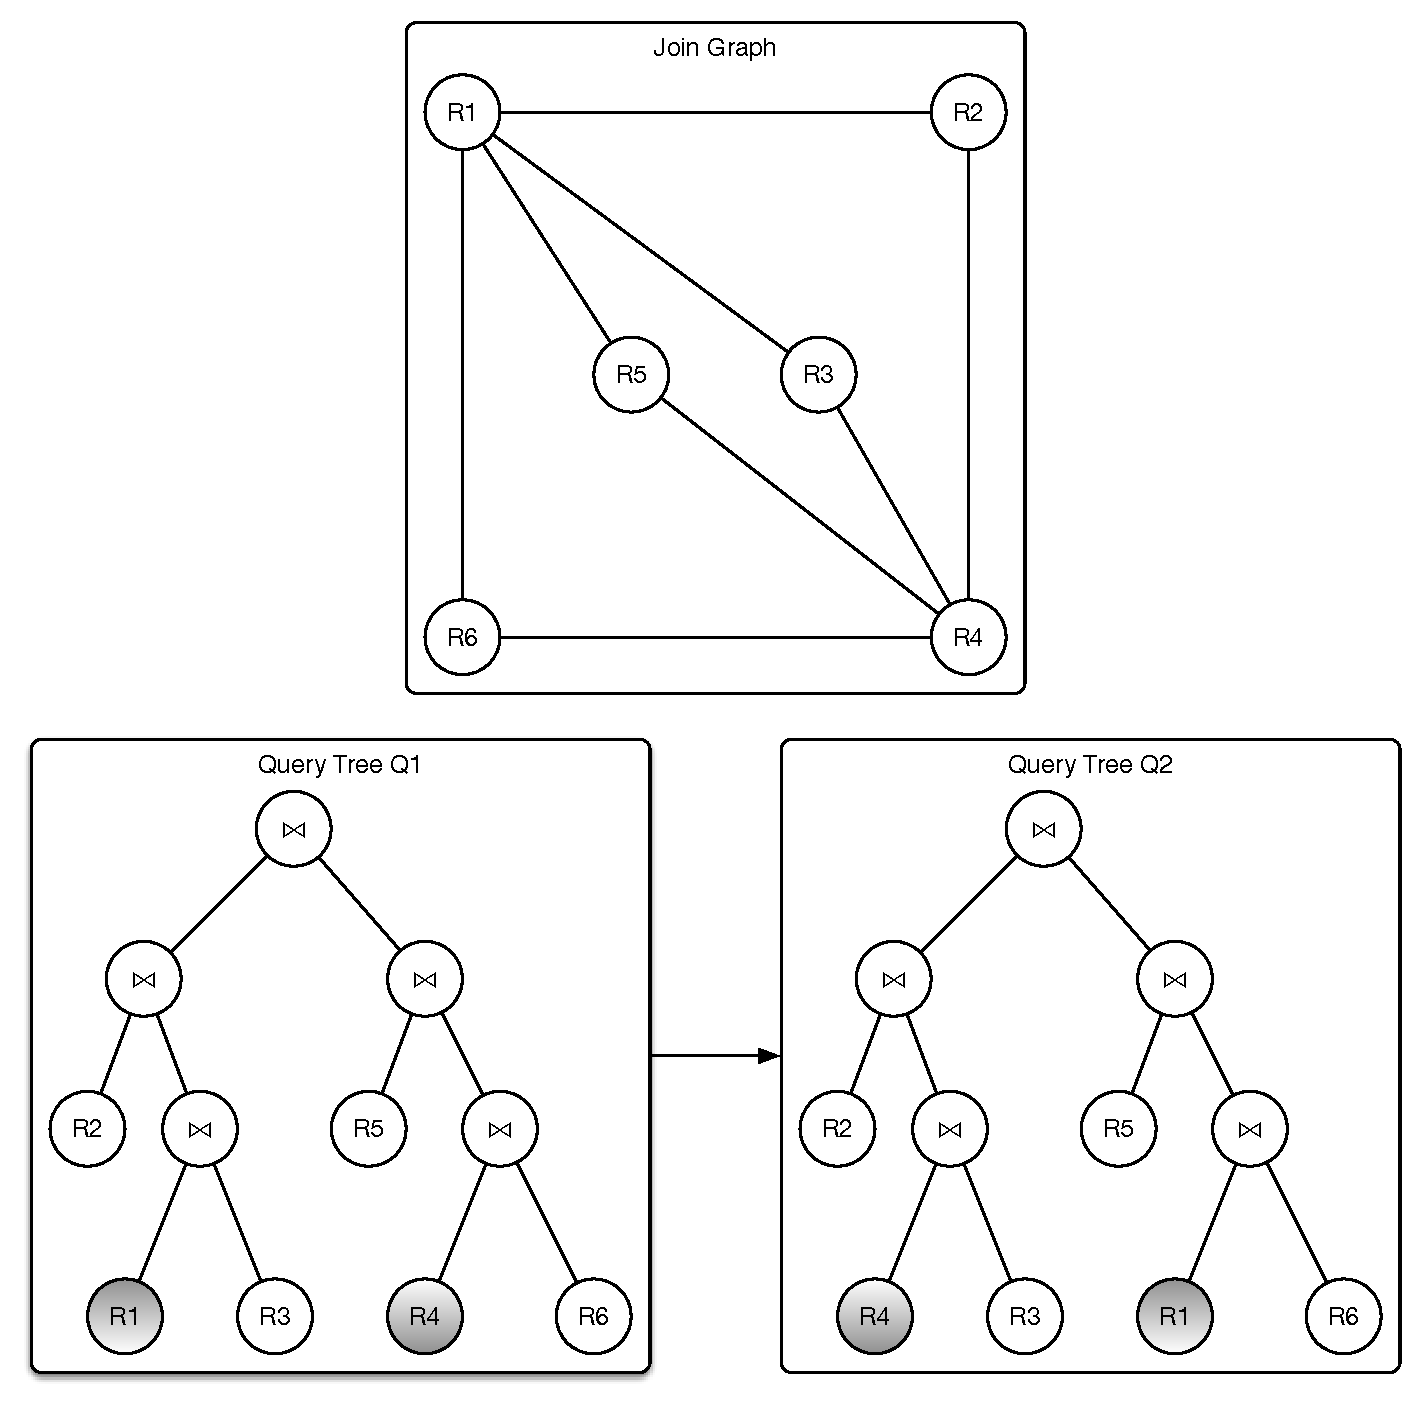
\includegraphics[width=\textwidth]{02_Related_Work/Graphs.pdf}
  \caption{Unvollständigkeit von RS-B2-CPS}
  \label{Incompleteness_RS-B2-CPS}
\end{figure}


Die Unvollständigkeit wurde mit Hilfe eines Beispiels belegt. Als Beispiel wurde der Bushy-Tree gewählt, der in Abbildung \ref{Incompleteness_RS-B2-CPS} zu sehen ist. Mit Hilfe der Regeln aus der Regelmenge RS-B2 sollte der initiale Plan (Q1) in den Plan (Q2) umgewandelt werden. Es wird versucht,  mit allen Regeln, der Regelmenge RS-B2 den Baum so zu transformieren, dass der gewünschte Zustand entsteht.

Zuerst soll der Baum mit der Kommutativitätsregel transformiert werden. Bei der Anwendung der Regel auf alle Planknoten wird klar, dass nur eine Kopie des Baums erzeugt werden kann, der den Baum spiegelt.

Durch die Anwendung von rechter Assoziativität kann auch R1 und R4 nicht vertauscht werden. Wendet man beispielsweise rechte Assoziativität auf den obersten Join-Knoten an, so entsteht ein neuer Baum, der ähnlich dem Graphen Q1 ist. Dem neuen Graphen wird auf der linken Seite der Knoten R5 hinzugefügt, wobei R4 und R6 eine Ebene weiter nach oben rutschen. Da auf diesen Knoten nur noch die Kommutativitätsregel angewendet werden kann, ist es nicht möglich, trotz eines späteren Tausches von R1 und R4 mit Hilfe der Exchange Regeln den in Abbildung Q2 vorgesehenen Endzustand zu erreichen. Auch eine Anwendung der Regel auf die untergeordneten Sub-Bäume kann die R1 und R4 nicht vertauschen.

Für die Anwendung der Exchange Rule ist es notwendig, dass Q1 in der Form ist, dass der linke Subbaum die Form $(R2 \Join R3) \Join R1$ besitzt und die rechte Seite die Form $R4 \Join (R5 \Join R6)$. Da jedoch die Knoten R2 und R3 keine Verbindung zueinander haben, ist es auch nicht möglich die Regel auszuführen. Daher ist der Austausch nicht möglich.

Es ist zwar möglich R2 und R5, R2 und R6, R3 und R5 sowie R3 und R6 zu vertauschen indem die Exchange-Regel angewendet wird. So können zwar alternative Pläne erzeugt werden, jedoch durch die Abschaltung der Regeln auf den entsprechenden Join-Knotwen wird es unmöglich die Exchange-Regel so anzuwenden, dass R1 und R4 vertauscht werden.


Somit ist klar, dass RS-B2 nicht vollständig ist und der gesamte Suchraum nicht exploriert werden kann.





\subsection{Unvollständigkeit von RS-B2 mit Hilfe von PyroJ}

Die Unvollständigkeit wurde auch mit Hilfe von PyroJ gezeigt. Hierzu wurden für die Regeln RS-B1-CPS und RS-B2-CPS verwendet. Die Tests wurden mit sternförmigen Anfragen durchgeführt. In Tabelle \ref{pyroIncomplete} sind die Anzahl der Relationen, die verwendet wurden und die korrespondierende Anzahl der Operatoren-Knoten zu sehen, die durch die beiden Algorithmen generiert wurden. Es wird klar, dass mit RS-B2 erheblich weniger Knoten gefunden wurden. 

\begin{figure}[ht]
\centering

\begin{tabular}{|l|l|l|}
Relationen & RS-B2-CPS & RS-B1-CPS \\
5          & 43        & 75        \\
7          & 207       & 399       \\
9          & 1043      & 2067      \\
11         & 5143      & 10263 \\         
\end{tabular}
\caption{Operatorenknoten-Vergleich bei Sternförmigen initialen Plänen}
\label{pyroIncomplete}
\end{figure}


%Bei den Tests, die von \cite{bachelor} durchgeführt wurden, wurde außerdem festgestellt, dass für eine bestimmte Anfrage (Query 7 des TPC-DS Benchmarks ohne Aggregation) Gesamtkosten mit Hilfe von RS-B2 geschätzt wurden, die um den Faktor 1.86 höher sind als die von RS-B1 ermittelten.

Diese Ergebnisse werden in Kaptel 5 erneut aufgegriffen und überprüft.



